\section{A route through lines, and why it does not close}
\label{app:lines}

Before the argument of Secs.~\ref{sec:direct} and~\ref{sec:loglaw} was found, we followed a route that bounds the spread $P$ of Eq.~\eqref{eq:PwP} line by line, on the lines $w = \text{const}$. We record it because it is correct, it works for regular states, and the way it fails identified the strips.

\paragraph*{Line decomposition (proved).} On each line the conditional density $\varrho(v\mid w)$ is the blur of a one-dimensional measure, so its sharpness $\omega(w) = \sigma^2\E[s_v^2\mid w]$ lies in $(0,1]$ and $\E_w[\omega] = a$. Let $\tilde p(w) = p_W(w)\,\omega(w)/a$ be the marginal along $w$ weighted by sharpness, and $\bar u(w)$ the sharpness-weighted mean position on the line. Jensen's inequality on the lines and the Cram\'er--Rao inequality under $\tilde p$ give
\begin{equation}
P \geq \frac{x^2 J_{ww}}{a\,I(\tilde p)}, \qquad x = \E_{\tilde p}[\bar u'],
\end{equation}
where $I(\tilde p)$ is the Fisher information of $\tilde p$ and $x$ is close to one (we proved two bounds on $|x - 1|$). On 377 Gaussian mixtures, stored and adversarial, the bound held everywhere and was at least $0.76$ in the focused regime (Fig.~\ref{fig:chain}).

\paragraph*{The constant of the route (proved).} By Minkowski's inequality and a line-wise Cauchy--Schwarz bound,
\begin{equation}
a\,I(\tilde p) \leq (1 + \bar D)\,J_{ww},
\end{equation}
where $\bar D$ is an average over lines of the dispersion $\Var(\varphi\mid w)/\omega$ of $\varphi = \sigma^2(2H_{vv} - s_v^2)$. For Gaussian lines $\bar D \leq 2$. We also proved $\Var(\varphi\mid w) \leq (\sqrt{3/4} + 1.5\sqrt2)^2 = 8.92$ on every line; the largest value found was $4.42$.

\paragraph*{Why it does not close (proved for a lattice, numerical otherwise).} The ratio $a I(\tilde p)/J_{ww}$ has no uniform bound. For a periodic ripple lattice along $v$ it equals $4k_0^2$ to leading order in the ripple amplitude, independently of the amplitude (Fig.~\ref{fig:families}); normalised patches of the lattice and localised ripples behave the same way, while Gaussian mixtures stayed below $1.31$. These states are not counterexamples to a gap of order $\sigma$, since they keep $g \geq 6.8$; the route simply loses information there. The reason is that $\bar D$ is normalised by the shape information along $w$ only, which vanishes for a product state, so that a ripple of any amplitude gives $\bar D = 4k_0^2$ at fixed $\sigma$. Lemma~\ref{lem:heisenberg} normalises by the full $J_{ww}$ instead, which removes this defect. Following the lattice to its limit led to the strips of Sec.~\ref{sec:strips}.

\begin{figure}[t]
\centering
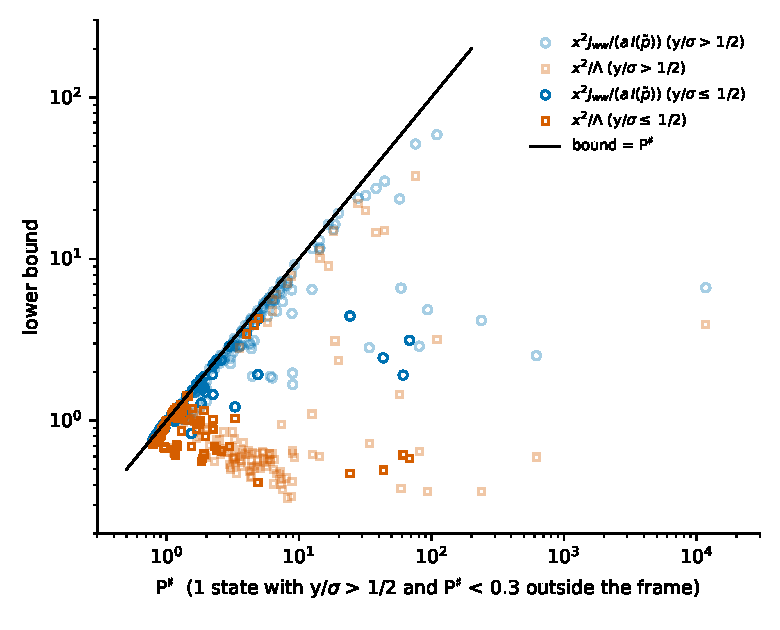
\includegraphics[width=0.85\columnwidth]{figures/figA1_chain.pdf}
\caption{The line route on 377 Gaussian mixtures: the lower bounds $x^2J_{ww}/(aI(\tilde p))$ (circles) and $x^2/\Lambda$ (squares) against the spread $P$ (denoted $P^\sharp$ in the axis label); dark symbols, focused states ($\Upsilon \leq 1/2$).}
\label{fig:chain}
\end{figure}

\begin{figure}[t]
\centering
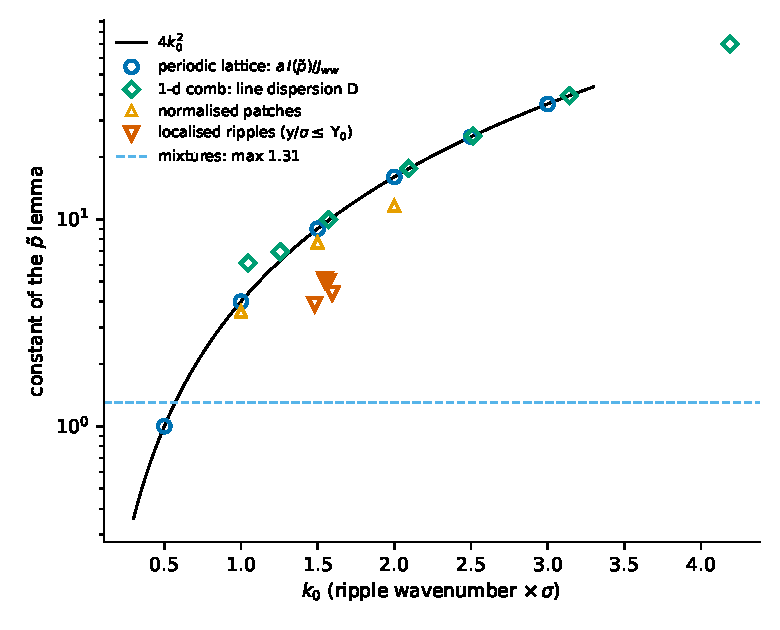
\includegraphics[width=0.85\columnwidth]{figures/figA2_families.pdf}
\caption{The constant of the line route on ripple families: periodic lattice and one-dimensional comb follow $4k_0^2$; normalised patches and localised ripples exceed the Gaussian-mixture maximum $1.31$ (dashed).}
\label{fig:families}
\end{figure}
